% vim: set fileencoding=utf-8 encoding=utf-8 tw=100:
\documentclass[spanish]{article}
\usepackage{babel}
\usepackage[utf8]{inputenc}
\usepackage{fullpage}
\usepackage{url}
\usepackage{palatino}
\usepackage{mathpazo}
\usepackage{amsmath}
\usepackage{amssymb}
\usepackage{cancel}
\usepackage{graphicx}

\newcommand{\pregunta}{\textit}
\newcommand{\given}{\vert}
\newcommand{\R}{\mathbb{R}}

\title{Reconocimiento de Patrones---Tarea 4}
\author{Roberto Bonvallet \\ \url {<rbonvall@gmail.com>}}
\date{Agosto de 2008}

\begin{document}
\maketitle

\section*{Pregunta 1}
\pregunta{
    Considere un conjunto de clases $\omega_i$, $i = 1, 2, \ldots, c$ y un conjunto de
    características representadas en el vector aleatorio $x$.  Sea $\omega_j$ tal que
    $P(\omega_j\given x)\ge P(\omega_i\given x)$ para todo $i = 1, 2, \ldots, c$.
}
\begin{enumerate}
    \item \pregunta{Muestre que $P(\omega_j\given x) \ge 1/c$.}

        Sin pérdida de generalidad, supongamos que $j = 1$, es decir, $\omega_1$ es la clase con
        mayor posterior.
        \begin{align}
            P(\omega_1\given x)   &\ge P(\omega_j\given x) \qquad\forall j = 1,\ldots, c \\
            \sum_{j=1}^c P(\omega_1\given x) &\ge \sum_{j=1}^c P(\omega_j\given x) \\
            c P(\omega_1\given x) &\ge 1 \\
            P(\omega_1\given x) &\ge 1/c 
        \end{align}

    \item \pregunta{Muestre que el mínimo error de clasificación está acotado por $(c - 1)/c$.}
        \begin{align}
            P(\text{error}) &= 1 - P(\text{correct}) \\
                &= 1 - \int_{\R^d} P(\text{correct}\given x)\,p(x)\,dx \\
                &= 1 - \int_{\R^d} \max_j \bigl\{ P(\omega_j\given x)\bigr\}\,p(x)\,dx \\
                &= 1 - \int_{\R^d} P(\omega_1\given x)\,p(x)\,dx \\
                &\le 1 - \frac{1}{c} \int_{\R^d} p(x)\,dx \\
                &= 1 - 1/c = (c - 1)/c
        \end{align}

    \item \pregunta{Describa la situación para la cual la cota anterior es una igualdad.}

        La igualdad se obtiene cuando $P(\text{correct}) = 1/c$.  Esto ocurre cuando
        $P(\omega_1\given x) = 1/c$, ya que la regla de decisión asigna siempre a $\omega_1$.

        Nuevamente sin pérdida de generalidad, supongamos que $P(\omega_2\given x_0)\ge
        P(\omega_i\given x_0)$ para todo $j = 2, \cdots, c$, en un punto $x = x_0$ en el espacio de
        características:
        \begin{align}
                \frac{c - 1}{c} = \sum_{j=2}^c P(\omega_j\given x_0) 
                &\le (c - 1)\,P(\omega_2\given x_0) \le (c - 1)\,P(\omega_1\given x_0) \\
                \frac{1}{c} &\le P(\omega_2\given x_0) \le \frac{1}{c} \\
                P(\omega_2\given x_0) &= \frac{1}{c}
        \end{align}
        El argumento no depende de la elección de $x_0$ y se puede repetir para $j = 3,\ldots, c$.
        Luego, en esta situación todas las clases tienen la misma posterior, igual a $1/c$.
\end{enumerate}

\section*{Pregunta 2}
\pregunta{
    Sea $p(x\given\omega_j)\sim N(\mu, \Sigma)$, $i = 1, 2$, la verosimilitud correspondiente a cada
    una de las clases de un problema de clasificación $d$-dimensional con las mismas matrices de
    covarianza pero con medias y a prioris arbitrarios.  Defina la distancia de Mahalanobis, $r_i$,
    mediante $r_i^2 = (x - \mu_j)^T \Sigma^{-1} (x - \mu)$.
}
\begin{enumerate}
    \item \pregunta{Muestre que en cualquier punto de la línea que une $\mu_1$ con $\mu_2$, los
        gradientes $\nabla r_1^2$ y $\nabla r_2^2$ apuntan en direcciones opuestas.}

        Usando las identidades $\nabla(y^T x) = y$ y $\nabla(x^T Ax) = 2Ax$, para $A$ simétrica, se
        tiene:
        \begin{align}
            \nabla r_j^2 &= \nabla (x^T\Sigma^{-1}x - 2\mu_j^T\Sigma^{-1}x + \mu_j^T\Sigma^{-1}\mu_j) \\
                         &= 2\Sigma^{-1}x - 2\Sigma^{-1}\mu_ j \\
                         &= 2\Sigma^{-1} (x - \mu_j)
        \end{align}
        La línea que une $\mu_1$ y $\mu_2$ se puede parametrizar como $x = t\mu_1 + (1 - t)\mu_2$,
        con $0\le t\le 1$.  Evaluando para ambas clases:
        \begin{align}
            \nabla r_1^2\bigl(t\mu_1 + (1 - t)\mu_2\bigr)
                &= 2\Sigma^{-1}\bigl(t\mu_1 + (1 - t)\mu_2 - \mu_1)\bigr) \\
                &= 2 (1 - t)\Sigma^{-1} (\mu_2 - \mu_1) \\
            \nabla r_2^2\bigl(t\mu_1 + (1 - t)\mu_2\bigr)
                &= 2\Sigma^{-1}\bigl(t\mu_1 + (1 - t)\mu_2 - \mu_1)\bigr) \\
                &= -2t\Sigma^{-1} (\mu_2 - \mu_1)
        \end{align}
        Como $t$ y $(1 - t)$ son positivos, ambos gradientes apuntan en direcciones opuestas.

    \item \pregunta{Muestre que el hiperplano separador óptimo es tangente a los hiperelipsoides de
        densidad de probabilidad constante en el punto en que dicho hiperplano corta la línea que une 
        $\mu_1$ con $\mu_2$.}

        Los hiperelipsoides de densidad de probabilidad constante son superficies de nivel de la
        función $r_j^2 = (x - \mu_j)^T \Sigma^{-1} (x - \mu_j)$ [Duda, \S2.5.2].  El vector normal a
        estas superficies es el gradiente $\nabla r_j^2$.  Del desarrollo anterior, sabemos que $\nabla
        r_j^2$ es proporcional a $\Sigma^{-1}(\mu_2 - \mu_1)$ sobre la línea que une las medias,
        para $j = 1$ y $j = 2$.

        La ecuación del hiperplano separador es $\bigl(\Sigma^{-1}(\mu_1 - \mu_2)\bigr)^T(x - x_0) = 0$
        [Duda, \S2.6.2, eqs.~61 y 62],
        donde $x_0$ es el punto de intersección con la línea que une las medias.
        El vector normal al plano es $\Sigma^{-1}(\mu_1 - \mu_2)$, como se ve directamente en la
        ecuación, y por lo tanto es paralelo a $\nabla r_j^2$ en $x_0$.

        Por lo tanto, el plano separador es tangente a los elipsoides de nivel de
        $p(x\given\omega_j)$ en $x_0$.

    \item \pregunta{Verdadero o falso: ``la frontera de decisión de un clasificador bayesiano
        corresponde en este problema al conjunto de puntos de igual distancia de Mahalanobis desde
        las respectivas medias''.  Justifique.}

        En el caso general, la frontera de decisión depende de las probabilidades a priori.  La
        distancia de Mahalanobis sólo es función de la verosimilitud (geometría de los clústers),
        por lo que no puede determinar unívocamente la frontera de decisión;  por lo tanto, la
        proposición es falsa.
\end{enumerate}

\section*{Pregunta 3}
\pregunta{Considere un problema de clasificación binario con a prioris idénticos. Demuestre
    %formalmente
    que el error de un clasificador bayesiano decrece (o no aumenta) si aumentamos el
    número de dimensiones del vector de características $x$.  Esto significa que no podemos reducir
    el error proyectando a un subespacio de menor dimensión.  Aun con este resultado en mano,
    explique por qué no es conveniente aumentar sin límites el número de características.}

    El error de un clasificador binario, con $P(\omega_1) = P(\omega_2) = 1/2$, está dado por:
    \begin{align}
        \text{Error}
        &= \int_{\R^d} P(\text{error}\given x)\, p(x)\, dx \\
        &= \int_{\R^d} \min\bigl\{
                P(\omega_1\given x), P(\omega_2\given x)
           \bigr\}\, p(x)\, dx \\
        &= \int_{\R^d} \min\left\{
                \frac{p(x\given\omega_1)}{\cancel{p(x)}}\cdot
                \frac{1}{2},
                \frac{p(x\given\omega_2)}{\cancel{p(x)}}\cdot
                \frac{1}{2}
           \right\}\, \cancel{p(x)}\, dx \\
        &\propto 
           \int_{\mathcal{R}_1} p(x\given\omega_1)\, dx +
           \int_{\mathcal{R}_2} p(x\given\omega_2)\, dx.
    \end{align}
    La frontera de decisión $\mathcal{S}$ es una hipersuperficie $\R^{d-1}$-dimensional que
    particiona a $\R^d$ de acuerdo a la verosimilitud de las clases.

    Al proyectar las características a un espacio $\R^{d-1}$-dimensional, la frontera de decisión
    pasa a ser una hipersuperficie $\R^{d-2}$-dimensional $\mathcal{S}'$.
    Al tener un grado de libertad menos, $\mathcal{S}'$ no puede corresponder a una superficie
    arbitraria en $\R^d$, y por lo tanto en general no coincide con $\mathcal{S}$.  Como
    $\mathcal{S}$ es la frontera que minimiza el error de Bayes, la frontera $\mathcal{S}'$ tiene
    que entregar un error igual o mayor.  En la figura siguiente, los vectores en las zonas
    punteadas quedarían mal clasificados por la frontera definida en el espacio proyectado:
    \begin{center}
        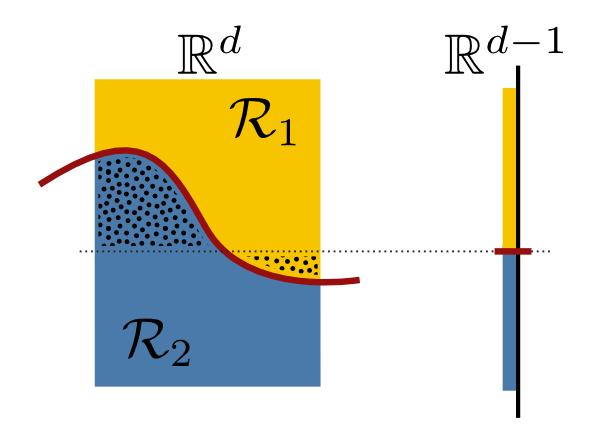
\includegraphics[width=0.3\textwidth]{error.png}
    \end{center}

   En general, nunca es buena idea aumentar indiscriminadamente el número de dimensiones, por los
   efectos indeseables que esto acarrea:
   \begin{itemize}
       \item \emph{maldición de la dimensionalidad:} el volumen del dominio aumenta exponencialmente
           con el número de dimensiones, lo que hace que puntos cercanos se alejen al aumentar las
           dimensiones, y que sean necesarias muestras mucho más grandes para cubrir una parte del
           espacio;  un efecto poco intutivo de esto es que el volumen de la hiperesfera unitaria se
           hace insignificante con respecto al del hipercubo unitario, por lo que la mayoría de los
           puntos del hipercubo quedan lejos del centro;
       \item el número de elementos de las matrices crece cuadráticamente respecto al número de
           dimensiones, por lo que los algoritmos pueden volverse prohibitivos en uso de recursos
           computacionales y de tiempo;
       \item \emph{principio de parsimonia:} en general los modelos más simples son preferibles a
           los complicados;
       \item agregar más características no hace que ellas sean significativas en el resultado de la
           clasificación: pueden ser totalmente irrelevantes o su aporte puede estar correlacionado
           con el que hacen otras características de mayor peso;
       \item como consecuencia de lo anterior, agregar dimensiones dependientes de otras puede
           introducir singularidades o mal condicionamiento en las ecuaciones que definen el modelo.
   \end{itemize}
\end{document}
